
%% bare_conf.tex
%% V1.3
%% 2007/01/11
%% by Michael Shell
%% See:
%% http://www.michaelshell.org/
%% for current contact information.
%%
%% This is a skeleton file demonstrating the use of IEEEtran.cls
%% (requires IEEEtran.cls version 1.7 or later) with an IEEE conference paper.
%%
%% Support sites:
%% http://www.michaelshell.org/tex/ieeetran/
%% http://www.ctan.org/tex-archive/macros/latex/contrib/IEEEtran/
%% and
%% http://www.ieee.org/

%%*************************************************************************
%% Legal Notice:
%% This code is offered as-is without any warranty either expressed or
%% implied; without even the implied warranty of MERCHANTABILITY or
%% FITNESS FOR A PARTICULAR PURPOSE! 
%% User assumes all risk.
%% In no event shall IEEE or any contributor to this code be liable for
%% any damages or losses, including, but not limited to, incidental,
%% consequential, or any other damages, resulting from the use or misuse
%% of any information contained here.
%%
%% All comments are the opinions of their respective authors and are not
%% necessarily endorsed by the IEEE.
%%
%% This work is distributed under the LaTeX Project Public License (LPPL)
%% ( http://www.latex-project.org/ ) version 1.3, and may be freely used,
%% distributed and modified. A copy of the LPPL, version 1.3, is included
%% in the base LaTeX documentation of all distributions of LaTeX released
%% 2003/12/01 or later.
%% Retain all contribution notices and credits.
%% ** Modified files should be clearly indicated as such, including **
%% ** renaming them and changing author support contact information. **
%%
%% File list of work: IEEEtran.cls, IEEEtran_HOWTO.pdf, bare_adv.tex,
%% bare_conf.tex, bare_jrnl.tex, bare_jrnl_compsoc.tex
%%*************************************************************************

% *** Authors should verify (and, if needed, correct) their LaTeX system ***
% *** with the testflow diagnostic prior to trusting their LaTeX platform ***
% *** with production work. IEEE's font choices can trigger bugs that do ***
% *** not appear when using other class files. ***
% The testflow support page is at:
% http://www.michaelshell.org/tex/testflow/



% Note that the a4paper option is mainly intended so that authors in
% countries using A4 can easily print to A4 and see how their papers will
% look in print - the typesetting of the document will not typically be
% affected with changes in paper size (but the bottom and side margins will).
% Use the testflow package mentioned above to verify correct handling of
% both paper sizes by the user's LaTeX system.
%
% Also note that the "draftcls" or "draftclsnofoot", not "draft", option
% should be used if it is desired that the figures are to be displayed in
% draft mode.
%
\documentclass[conference]{IEEEtran}
% Add the compsoc option for Computer Society conferences.
%
% If IEEEtran.cls has not been installed into the LaTeX system files,
% manually specify the path to it like:
% \documentclass[conference]{../sty/IEEEtran}

\usepackage{graphicx}
\usepackage{datetime}
\usepackage{cite}
\usepackage[hyphens]{url}
\usepackage[hidelinks]{hyperref}
\usepackage{csquotes}
\usepackage{array}
\usepackage {adjustbox}
\usepackage{tcolorbox}
\usepackage{graphicx}
\usepackage{multirow}
\usepackage{multicol}
\usepackage{pdflscape}
\usepackage{amsmath}
\usepackage{float}
\usepackage{afterpage}
\graphicspath{ {images/} }
\hypersetup{breaklinks=true}
\newcommand{\subparagraph}{}
\usepackage{titlesec}
\setcounter{secnumdepth}{4}

% Some very useful LaTeX packages include:
% (uncomment the ones you want to load)


% *** MISC UTILITY PACKAGES ***
%
%\usepackage{ifpdf}
% Heiko Oberdiek's ifpdf.sty is very useful if you need conditional
% compilation based on whether the output is pdf or dvi.
% usage:
% \ifpdf
% % pdf code
% \else
% % dvi code
% \fi
% The latest version of ifpdf.sty can be obtained from:
% http://www.ctan.org/tex-archive/macros/latex/contrib/oberdiek/
% Also, note that IEEEtran.cls V1.7 and later provides a builtin
% \ifCLASSINFOpdf conditional that works the same way.
% When switching from latex to pdflatex and vice-versa, the compiler may
% have to be run twice to clear warning/error messages.






% *** CITATION PACKAGES ***
%
%\usepackage{cite}
% cite.sty was written by Donald Arseneau
% V1.6 and later of IEEEtran pre-defines the format of the cite.sty package
% \cite{} output to follow that of IEEE. Loading the cite package will
% result in citation numbers being automatically sorted and properly
% "compressed/ranged". e.g., [1], [9], [2], [7], [5], [6] without using
% cite.sty will become [1], [2], [5]--[7], [9] using cite.sty. cite.sty's
% \cite will automatically add leading space, if needed. Use cite.sty's
% noadjust option (cite.sty V3.8 and later) if you want to turn this off.
% cite.sty is already installed on most LaTeX systems. Be sure and use
% version 4.0 (2003-05-27) and later if using hyperref.sty. cite.sty does
% not currently provide for hyperlinked citations.
% The latest version can be obtained at:
% http://www.ctan.org/tex-archive/macros/latex/contrib/cite/
% The documentation is contained in the cite.sty file itself.






% *** GRAPHICS RELATED PACKAGES ***
%
\ifCLASSINFOpdf
% \usepackage[pdftex]{graphicx}
% declare the path(s) where your graphic files are
% \graphicspath{{../pdf/}{../jpeg/}}
% and their extensions so you won't have to specify these with
% every instance of \includegraphics
% \DeclareGraphicsExtensions{.pdf,.jpeg,.png}
\else
% or other class option (dvipsone, dvipdf, if not using dvips). graphicx
% will default to the driver specified in the system graphics.cfg if no
% driver is specified.
% \usepackage[dvips]{graphicx}
% declare the path(s) where your graphic files are
% \graphicspath{{../eps/}}
% and their extensions so you won't have to specify these with
% every instance of \includegraphics
% \DeclareGraphicsExtensions{.eps}
\fi
% graphicx was written by David Carlisle and Sebastian Rahtz. It is
% required if you want graphics, photos, etc. graphicx.sty is already
% installed on most LaTeX systems. The latest version and documentation can
% be obtained at: 
% http://www.ctan.org/tex-archive/macros/latex/required/graphics/
% Another good source of documentation is "Using Imported Graphics in
% LaTeX2e" by Keith Reckdahl which can be found as epslatex.ps or
% epslatex.pdf at: http://www.ctan.org/tex-archive/info/
%
% latex, and pdflatex in dvi mode, support graphics in encapsulated
% postscript (.eps) format. pdflatex in pdf mode supports graphics
% in .pdf, .jpeg, .png and .mps (metapost) formats. Users should ensure
% that all non-photo figures use a vector format (.eps, .pdf, .mps) and
% not a bitmapped formats (.jpeg, .png). IEEE frowns on bitmapped formats
% which can result in "jaggedy"/blurry rendering of lines and letters as
% well as large increases in file sizes.
%
% You can find documentation about the pdfTeX application at:
% http://www.tug.org/applications/pdftex





% *** MATH PACKAGES ***
%
%\usepackage[cmex10]{amsmath}
% A popular package from the American Mathematical Society that provides
% many useful and powerful commands for dealing with mathematics. If using
% it, be sure to load this package with the cmex10 option to ensure that
% only type 1 fonts will utilized at all point sizes. Without this option,
% it is possible that some math symbols, particularly those within
% footnotes, will be rendered in bitmap form which will result in a
% document that can not be IEEE Xplore compliant!
%
% Also, note that the amsmath package sets \interdisplaylinepenalty to 10000
% thus preventing page breaks from occurring within multiline equations. Use:
%\interdisplaylinepenalty=2500
% after loading amsmath to restore such page breaks as IEEEtran.cls normally
% does. amsmath.sty is already installed on most LaTeX systems. The latest
% version and documentation can be obtained at:
% http://www.ctan.org/tex-archive/macros/latex/required/amslatex/math/





% *** SPECIALIZED LIST PACKAGES ***
%
%\usepackage{algorithmic}
% algorithmic.sty was written by Peter Williams and Rogerio Brito.
% This package provides an algorithmic environment fo describing algorithms.
% You can use the algorithmic environment in-text or within a figure
% environment to provide for a floating algorithm. Do NOT use the algorithm
% floating environment provided by algorithm.sty (by the same authors) or
% algorithm2e.sty (by Christophe Fiorio) as IEEE does not use dedicated
% algorithm float types and packages that provide these will not provide
% correct IEEE style captions. The latest version and documentation of
% algorithmic.sty can be obtained at:
% http://www.ctan.org/tex-archive/macros/latex/contrib/algorithms/
% There is also a support site at:
% http://algorithms.berlios.de/index.html
% Also of interest may be the (relatively newer and more customizable)
% algorithmicx.sty package by Szasz Janos:
% http://www.ctan.org/tex-archive/macros/latex/contrib/algorithmicx/




% *** ALIGNMENT PACKAGES ***
%
%\usepackage{array}
% Frank Mittelbach's and David Carlisle's array.sty patches and improves
% the standard LaTeX2e array and tabular environments to provide better
% appearance and additional user controls. As the default LaTeX2e table
% generation code is lacking to the point of almost being broken with
% respect to the quality of the end results, all users are strongly
% advised to use an enhanced (at the very least that provided by array.sty)
% set of table tools. array.sty is already installed on most systems. The
% latest version and documentation can be obtained at:
% http://www.ctan.org/tex-archive/macros/latex/required/tools/


%\usepackage{mdwmath}
%\usepackage{mdwtab}
% Also highly recommended is Mark Wooding's extremely powerful MDW tools,
% especially mdwmath.sty and mdwtab.sty which are used to format equations
% and tables, respectively. The MDWtools set is already installed on most
% LaTeX systems. The lastest version and documentation is available at:
% http://www.ctan.org/tex-archive/macros/latex/contrib/mdwtools/


% IEEEtran contains the IEEEeqnarray family of commands that can be used to
% generate multiline equations as well as matrices, tables, etc., of high
% quality.


%\usepackage{eqparbox}
% Also of notable interest is Scott Pakin's eqparbox package for creating
% (automatically sized) equal width boxes - aka "natural width parboxes".
% Available at:
% http://www.ctan.org/tex-archive/macros/latex/contrib/eqparbox/





% *** SUBFIGURE PACKAGES ***
%\usepackage[tight,footnotesize]{subfigure}
% subfigure.sty was written by Steven Douglas Cochran. This package makes it
% easy to put subfigures in your figures. e.g., "Figure 1a and 1b". For IEEE
% work, it is a good idea to load it with the tight package option to reduce
% the amount of white space around the subfigures. subfigure.sty is already
% installed on most LaTeX systems. The latest version and documentation can
% be obtained at:
% http://www.ctan.org/tex-archive/obsolete/macros/latex/contrib/subfigure/
% subfigure.sty has been superceeded by subfig.sty.



%\usepackage[caption=false]{caption}
%\usepackage[font=footnotesize]{subfig}
% subfig.sty, also written by Steven Douglas Cochran, is the modern
% replacement for subfigure.sty. However, subfig.sty requires and
% automatically loads Axel Sommerfeldt's caption.sty which will override
% IEEEtran.cls handling of captions and this will result in nonIEEE style
% figure/table captions. To prevent this problem, be sure and preload
% caption.sty with its "caption=false" package option. This is will preserve
% IEEEtran.cls handing of captions. Version 1.3 (2005/06/28) and later 
% (recommended due to many improvements over 1.2) of subfig.sty supports
% the caption=false option directly:
%\usepackage[caption=false,font=footnotesize]{subfig}
%
% The latest version and documentation can be obtained at:
% http://www.ctan.org/tex-archive/macros/latex/contrib/subfig/
% The latest version and documentation of caption.sty can be obtained at:
% http://www.ctan.org/tex-archive/macros/latex/contrib/caption/




% *** FLOAT PACKAGES ***
%
%\usepackage{fixltx2e}
% fixltx2e, the successor to the earlier fix2col.sty, was written by
% Frank Mittelbach and David Carlisle. This package corrects a few problems
% in the LaTeX2e kernel, the most notable of which is that in current
% LaTeX2e releases, the ordering of single and double column floats is not
% guaranteed to be preserved. Thus, an unpatched LaTeX2e can allow a
% single column figure to be placed prior to an earlier double column
% figure. The latest version and documentation can be found at:
% http://www.ctan.org/tex-archive/macros/latex/base/



%\usepackage{stfloats}
% stfloats.sty was written by Sigitas Tolusis. This package gives LaTeX2e
% the ability to do double column floats at the bottom of the page as well
% as the top. (e.g., "\begin{figure*}[!b]" is not normally possible in
% LaTeX2e). It also provides a command:
%\fnbelowfloat
% to enable the placement of footnotes below bottom floats (the standard
% LaTeX2e kernel puts them above bottom floats). This is an invasive package
% which rewrites many portions of the LaTeX2e float routines. It may not work
% with other packages that modify the LaTeX2e float routines. The latest
% version and documentation can be obtained at:
% http://www.ctan.org/tex-archive/macros/latex/contrib/sttools/
% Documentation is contained in the stfloats.sty comments as well as in the
% presfull.pdf file. Do not use the stfloats baselinefloat ability as IEEE
% does not allow \baselineskip to stretch. Authors submitting work to the
% IEEE should note that IEEE rarely uses double column equations and
% that authors should try to avoid such use. Do not be tempted to use the
% cuted.sty or midfloat.sty packages (also by Sigitas Tolusis) as IEEE does
% not format its papers in such ways.





% *** PDF, URL AND HYPERLINK PACKAGES ***
%
%\usepackage{url}
% url.sty was written by Donald Arseneau. It provides better support for
% handling and breaking URLs. url.sty is already installed on most LaTeX
% systems. The latest version can be obtained at:
% http://www.ctan.org/tex-archive/macros/latex/contrib/misc/
% Read the url.sty source comments for usage information. Basically,
% \url{my_url_here}.





% *** Do not adjust lengths that control margins, column widths, etc. ***
% *** Do not use packages that alter fonts (such as pslatex). ***
% There should be no need to do such things with IEEEtran.cls V1.6 and later.
% (Unless specifically asked to do so by the journal or conference you plan
% to submit to, of course. )


% correct bad hyphenation here
\hyphenation{op-tical net-works semi-conduc-tor}


\begin{document}
%
% paper title
% can use linebreaks \\ within to get better formatting as desired
%\title{On the Impact of Security Questions on Answers}
%\title{``secret question meter": A visual interface design nudges users towards stronger answers in security questions}
\title{%
A model for measuring perceived privacy of users for system designers }
% author names and affiliations
% use a multiple column layout for up to three different
% affiliations

%\author{\IEEEauthorblockN{Awanthika Rasanjalee Senarath\IEEEauthorrefmark{1},
%and Nalin A.G. Arachchilage \IEEEauthorrefmark{2} }
%\IEEEauthorblockA{Australian Centre for Cyber Security\\
%University of New South Wales Canberra\\
%Australian Defence Force Academy\\
%Email: \IEEEauthorrefmark{1}a.senarath@student.unsw.edu.au,
%\IEEEauthorrefmark{2}nalin.asanka@adfa.edu.au
%}}




% conference papers do not typically use \thanks and this command
% is locked out in conference mode. If really needed, such as for
% the acknowledgment of grants, issue a \IEEEoverridecommandlockouts
% after \documentclass

% for over three affiliations, or if they all won't fit within the width
% of the page, use this alternative format:
% 
%\author{\IEEEauthorblockN{Michael Shell\IEEEauthorrefmark{1},
%Homer Simpson\IEEEauthorrefmark{2},
%James Kirk\IEEEauthorrefmark{3}, 
%Montgomery Scott\IEEEauthorrefmark{3} and
%Eldon Tyrell\IEEEauthorrefmark{4}}
%\IEEEauthorblockA{\IEEEauthorrefmark{1}School of Electrical and Computer Engineering\\
%Georgia Institute of Technology,
%Atlanta, Georgia 30332--0250\\ Email: see http://www.michaelshell.org/contact.html}
%\IEEEauthorblockA{\IEEEauthorrefmark{2}Twentieth Century Fox, Springfield, USA\\
%Email: homer@thesimpsons.com}
%\IEEEauthorblockA{\IEEEauthorrefmark{3}Starfleet Academy, San Francisco, California 96678-2391\\
%Telephone: (800) 555--1212, Fax: (888) 555--1212}
%\IEEEauthorblockA{\IEEEauthorrefmark{4}Tyrell Inc., 123 Replicant Street, Los Angeles, California 90210--4321}}




% use for special paper notices
%\IEEEspecialpapernotice{(Invited Paper)}




% make the title area
\maketitle

\begin{abstract}
%\boldmath
Users are known to be reluctant to disclose their data into software systems when their perceived privacy risk of disclosing data into a software system is high. Understanding this perceived privacy risk and making use of it when implementing software systems could help building software systems that could reduce the perceived privacy risk of users. In this paper, we attempt to build a model that could be used to measure the perceived privacy risk of users in general when they disclose data into a given software system. We first derive a model to measure the perceived privacy risk based on existing knowledge and then we test our model through a survey with 151 participants. The final model we derived showed that how visible data gets in an application by default when the user discloses data into the application had the highest impact on the perceived privacy risk of users. 

\end{abstract}
% IEEEtran.cls defaults to using nonbold math in the Abstract.
% This preserves the distinction between vectors and scalars. However,
% if the conference you are submitting to favors bold math in the abstract,
% then you can use LaTeX's standard command \boldmath at the very start
% of the abstract to achieve this. Many IEEE journals/conferences frown on
% math in the abstract anyway.

% no keywords

% For peer review papers, you can put extra information on the cover
% page as needed:
% \ifCLASSOPTIONpeerreview
% \begin{center} \bfseries EDICS Category: 3-BBND \end{center}
% \fi
%
% For peerreview papers, this IEEEtran command inserts a page break and
% creates the second title. It will be ignored for other modes.
\IEEEpeerreviewmaketitle


 

\section{Introduction}



Disclosure of personal details into software systems always comes with an associated privacy risk  \cite {malhotra2004internet} and the data disclosure decisions of users are closely related to their perceived privacy risk \cite {li2010understanding}. That is, users are most likely to disclose data to a software system if they feel that the ways through which the system could compromise their privacy (data sharing, data selling) from the data they disclose is minimum  \cite {kobsa2007privacy}. Hence, understanding data disclosure decisions made by users in a given circumstance could help understanding the perceived privacy risk by users. Understanding this perceived privacy risk of users when they interact with software systems is imortant to enhance users satisfaction in data disclosure as well as designing systems to ensure the privacy risk is appropriately handled by design. For example, it has been said that users are likely to feel more comfortable to share their data when they know how the system would use the data \cite {knijnenburg2013helping}. However, for this, it is essential that developers understand which data users would feel most uncomfortable sharing. Nevertheless, among many research that attempts to interpret users privacy risk and their data disclosure decisions \cite {knijnenburg2013making}, so far no attempt has been made to communicate this perceived privacy risk of users when they disclose data into systems, in a comprehensive way to software developers.


Previous research has identified that properties of the data (such as the user's name, address) being disclosed have an effect on data disclosure decisions made by users. For example, when a user discose data to a system, how sensitive is this data? and how relevant is this data to the application? are known to have an effect on the decision of the user to either disclose the data to the system or nots \cite {malheiros2013fairly}. Consequently, previous research has shown that the knowledge of the effect of the properties of data could help building up a metric for privacy risk of data items \cite {maximilien2009privacy} that could measure the privacy risk of content in software systems. Such a privacy metric that communicates the associated privacy risk of data items in a given scenario could help software developers to decide which data to collect, which data to store and how to communicate the use of data in a system when they design software systems in order to reduce the perceived privacy risk. Similarly, with a privacy measurement metric on data items researchers and law makers can make better regulations and privacy practices that would relate privacy with the user data.

Nevertheless, most of the previous approaches to observe decisions made by users when they disclose data into systems, focus either on the features of the system that requests data \cite {li2010understanding, wang2016context, malheiros2013fairly} or the personality of the user who discloses data \cite {nissenbaum2009privacy}. These research attempts to increase user data disclosure to collect and use more data in software systems \cite {dennett2000little}. In this research we focus on the effect of the properties of the data itself and the context in which the data is being disclosed on the privacy risk perceived by users when they disclose data into software systems. With this we  attempt to develop a privacy metric to measure the perceived privacy risk of users when they disclose data into different system settings. For this, building on previous knowledge on privacy risk measurement, we first develop a model to measure the privacy risk of data items in a given application context. Then, using a survey with 151 respondents we observe how good our model fits with the actual privacy risk perceived by users.

The paper is structured as follows. We first discuss the background of perceived privacy risk of users, and privacy risk measurement to establish the grounds on which our wor stand. Then, building on the existing theoretical knowledge on measuring privacy risk, we first logically build our model to measure user privacy risk associated with disclosing data items in a given software system setting. Then, we describe the experiment we conducted to measure actual privacy risk perceived by users when they disclose their data. Next, we present our results where we show how good out model fits the observations, followed by a discussion of the observed variations of our model. Finally, we present our conclusions and directions for future research

\section {Background}

Our focus in this research is to develop a metric to measure the perceived privacy risk of users when they disclose their data (such as their name, address and email address) into different application settings (such as their baking app, their social networking account etc.). For this we first analyzed the existing work that identify factors that affect data disclosure decisions of users when they use software systems. 

Most research that observe disclosure decisions of users attempt to identify factors that could increase user data disclosure. For example, Besmer et al. said that users are more likely to decide to disclose data when they are shown the decisions made by other users \cite {besmer2010impact} Similarly, Dennett has said that users feel comfortable sharing their data when they are shown the decisions made by their friends. \cite {dennett2000little}. Furthermore, Acquisti et al. found that changing the order of intrusiveness of the data being requested also makes users disclose more data when interacting with software systems \cite {acquisti2012impact}. Similarly, testing the effect of the justification provided by the system when requesting data Knijnenburg and Kobsa \cite {knijnenburg2013helping} revealed that when users are told \textit{this data is useful for you} users are more likely to disclose data with the application. Interestingly, all these research focus on system behaviors (way of requesting data, justification for data collection) and user's personal preferences ( users' experience with a system, users' expectation from a system) and their effects on user data disclosure decisions.

Consequently, focusing on the intrinsic properties of the data being shared, Bansal et al. have shown that users' intention to disclose health information is affected by the sensitivity of the data\cite {bansal2010impact}. This intrigued our interest. Malhotra et al. have also shown that consumer willingness to share personal data in commercial platforms is affected by the sensitivity of the data \cite {malhotra2004internet}. Similarly, Malheiros et al. \cite {malheiros2013fairly} have shown that sensitivity of data items such as date of birth and occupation had a significant affect on the decisions of the users to disclose that data into software systems. Interestingly, they have also identified an effect of data relevance for a given application context on disclosure decisions made by users. However, how these parameters correlate when user make their decisions to disclose data and how software developers could make use of this information when they design software systems are not yet known.

Interestingly, from a perspective of privacy risk measurement, Maximilien et al. \cite {maximilien2009privacy} have shown that a metric for privacy in a given context can be obtained by multiplying the measurement for sensitivity of a data item with the measurement for visibility the data item gets in an application. They define their metric for privacy as \enquote{a measurement that determines their [the user's ]willingness to disclose information associated with this item} \cite {maximilien2009privacy}. Using this metric, Minkus and Memon \cite{minkus2014scale} have attempted to measure user privacy from users' Facebook privacy settings. They have shown that the metric could be used to measure the privateness of a user from the choices s/he makes when setting up the privacy settings in Facebook. However, privacy risk is a contextual measurements. The context in which data is being disclosed \cite {nissenbaum2009privacy, john2010strangers} is known to have an effect on user disclosure decisions \cite {knijnenburg2013making}. For example, it is said that users have a negative attitude towards rewards for data disclosure when the requested data appears irrelevant for a system \cite {li2010understanding}, whereas they accepted the rewards if the data is relevant for the system. However, in the current metric for privacy risk measurement of content, this measurement of data relatedness is missing.

In this research, we focus on the effect of data sensitivity, the relevance of the data for an application and the visibility the data gets in the application on the perceived privacy risk of users. With this we focus on obtaining a privacy risk metric that could communicate the effect of data sensitivity, visibility and the relatedness of data for a particular application on the perceived privacy risk of users to software developers and privacy researchers. By software developers, we refer to all those who are involved in making the decisions on collecting data, designing and implementing the software system in an organization. This metric would help them to understand and incorporate perceived privacy risk of users into the software system designs and assist the development of privacy preserving software systems. For example, they could identify which data users are most concerned about and which data users would feel most uncomfortable sharing. This knowledge could help them implement better security for data in system designs and communicate it to the user in order to actively reduce the perceived privacy risk of users when they interact with software systems.


\section {Research Methodology}

In this section we first introduce the parameters of data we are interested in. Then using these parameters we derive and propose a model to measure privacy risk of data items based on existing theoretical knowledge.

\subsection {Model to calculate privacy risk of data elements}

The goal of our research was to develop a measurement to calculate the perceived privacy risk of users when they disclose data into software systems. Referring to previous research we identified data sensitivity (S), relatedness (R) and visibility (V) of data on the perceived privacy risk of users when they make the disclosure decisions. For the context of this research we define data sensitivity, visibility and relatedness of data to be parameters that depend only on a particular data item \textit{$D_i$} and the application context in which it is being used \textit{$C_j$}. Next, we define these parameters for the context of this research.

\subsubsection{Data Sensitivity} We define the sensitivity of a particular data item to be a parameter that is dependent on the data item \textit{$D_i$} itself. That is inherently for a user their credit card number is ore sensitive than their age. We define sesitivity of a data item to be the perceived impact of loss of that particular data item. We define sensitivity in three categorical values. These categories are defined based on the definition of sensitive data in the European Data Protection Regulations (GDPR) \cite {wagner2016national} and logical reasoning. We used three categories for this categorization as it is cognitively more manageable than complex scales with more levels of categorization \cite {oetzel2014systematic}. The categories we propose are presented in table I.  

\begin{center}
\begin{table}[htbp]
\caption{Data Sensitivity}
\begin{center}
\begin{adjustbox}{width=0.5\textwidth} 
\begin{tabular}{|p{0.2\linewidth}|p{0.7\linewidth}|p{0.1\linewidth}|} 
\hline
Category & Description & Sensitivity Value \\
\hline
Category I - Highest sensitivity & Data that could be used to identify a unique characteristic of a person. For example, a person's race, religion or HIV status. & 3 \\
\hline
Category II - Moderate sensitivity & Personally Identifiable information about the person. For example, a person's name, address, mobile number & 2 \\
\hline
Category III - Low sensitivity & Any other detail about a person that may have an impact of loss, however, would not affect the person. For example, a person's high school & 1 \\
\hline
\end{tabular}
\end{adjustbox}
\end{center}
\end{table}
\end{center} 

Therefore according to our definition the sensitivity of a data element \textit {$D_i$} takes categorical values \textit {$S_i$} $\in$ \{1,2,3\}.

\subsubsection {Data visibility} We define the visibility of a data element to be an inherent property gained by a particular data element \textit{$D_i$} in a particular application context \textit{$C_j$} due to the design of the application. That is how visible the data item would be by default once the user disclose the data item to the application. If the application by default allows the data to be seen only by the user, we define that data item has the lowest visibility. These categories are defined on the basis of the survey conducted by Minkus et al. \cite{minkus2014scale} in their attempts to scale Facebook privacy settings according to their visibility, they have asked participants questions that investigate the users perception of visibility of their content in Facebook. Building on their reasoning we logically form the three visibility categories presented in Table II.

\begin{center}
\begin{table}[htbp]
\caption{Data Visibility}
\begin{center}
\begin{adjustbox}{width=0.5\textwidth} 
\begin{tabular}{|p{0.2\linewidth}|p{0.7\linewidth}|p{0.1\linewidth}|} 
\hline
Category & Description & Visibility Value \\
\hline
Category I - Highest visibility & Data would be seen by any one by default. Data is visible in the application by default. For example the name of a user in Facebook & 3 \\
\hline
Category II - Moderate visibility & Data would be seen by a controlled set of users by default. For example, content that can be only see by the friends of the user in Facebook & 2 \\
\hline
Category III - Low visibility & Data would be seen by any one by default. Data is visible in the application by default. For example, your pin number in the banking app will not be visible to anyone & 1 \\
\hline
\end{tabular}
\end{adjustbox}
\end{center}
\end{table}
\end{center} 

Therefore according to our definition the visibility of a data element \textit {$D_i$} in an application context textit {$C_j$} takes categorical values \textit {$V_{i,j}$} $\in$ \{1,2,3\}.

\subsubsection {Data Relatedness} We define the relatedness of a data element \textit {$D_i$} to be a property that is defined by the application context \textit {$C_j$}. That is based on the requirements of the application, the data could be highly related to the application (For example, your bank account number for your banking application) or no related at all. This is determined by the primary functionality of the application defined by the application requirements. We build this categorization based on logical reasoning. While it has been widely accepted that the relatedness of data affects the privacy risk perceived by users when they disclose data into software systems, so far there is no evidence as to how related a data item should be in order to make users feel comfortable sharing those data into the system. Therefore, based on logical reasoning, we propose the categorization present in table III for scaling data relatedness to a software system. 

\begin{center}
\begin{table}[htbp]
\caption{Data Relatedness}
\begin{center}
\begin{adjustbox}{width=0.5\textwidth} 
\begin{tabular}{|p{0.2\linewidth}|p{0.7\linewidth}|p{0.1\linewidth}|} 
\hline
Category & Description & Relatedness Value \\
\hline
Category I - Highest relatedness & Data the application cannot do without. These data ara absolutely necessary for the primary functionality of the application & 3 \\
\hline
Category II - Moderate relatedness & Data could add additional functionality to the application. For example, data that could deliver benefits through data analysis techniques & 2 \\
\hline
Category III - Low relatedness & Data the application can do without. & 1 \\
\hline
\end{tabular}
\end{adjustbox}
\end{center}
\end{table}
\end{center} 
Therefore according to our definition the relatedness of a data element \textit {$D_i$} in an application context \textit {$C_j$} also takes categorical values \textit {$R_{i,j}$} $\in$ \{1,2,3\}.

\subsubsection {Model to calculate privacy risk of a data element \textit {$D_i$} in an application context \textit {$C_j$} }

We define the calculated privacy risk \textit{$P_c$} of a data element \textit {$D_i$} in an application context \textit {$C_j$} as follows.

Building up on the relationship proposed by Maximilien et al. \cite {maximilien2009privacy} we define that the privacy risk \textit{$P_c$} of a data element \textit {$D_i$} in an application context \textit {$C_j$}  monotonicall increases with the sensitivity of a data item \textit{$S_i$} and the visibility of a data item in a given context \textit{$V_{(i,j)}$}. This has been previously used by Minkus and Memon \cite{minkus2014scale} in determining the privacy level of Facebook privacy settings for a particular user. Based on this, we propose that the privacy risk \textit{$P_c$} of a data element \textit {$D_i$} in an application context \textit {$C_j$} is in a monotonically decremental relationship with the relatedness of the data element \textit {$D_i$} to the application context \textit {$C_j$}. This is based on the knowledge that users perceive low privacy risk when disclosing data items that are relevant to the application as opposed to data elements that do not appear relevant \cite {knijnenburg2013helping}. Therefore, we propose that an approximation for the privacy risk \textit{$P_c$} of a data element \textit {$D_i$} in an application context \textit {$C_j$} can be obtained by,

\[
\text {Privacy Risk $P_{(i,j)}$} =\frac{S_{i}^a \times V_{(i,j)}^b}{R_{(i,j)}^ c}
\]

where a,b and c values could take any real number. However, as we are aiming for an approximation we limit a,b,c to whole numbers.

According to this calculation Privacy Risk $P_{(i,j)}$  of a data element \textit {$D_i$} in an application context \textit {$C_j$} $\in$ \{x$\mid$ x $in$ ${\rm I\!R}$ where, 0 $\leq$ x\}. This relationship could be used to measure the privacy risk of data in a given application context so that developers and system designers could get an idea as to how appropriate privacy measures should be implemented for data items in an application design. We argue that this numeric measurement of privacy measurement would be meaningful for software developers that the soft measurements developers are expected to make in most scenarios that involve user privacy. For example, it has been previously coined that when implementing privacy in software systems, developers find it difficult to interpret the requirements to anonymize appropriate data, encrypt sensitive data, when decisions are not measurable \cite {senarath2018why}. 



Next, in order to see how closely the proposed model fit the actual perceived privacy risk of users when they disclose data we conducted a survey study.

\subsection {Research Study}

Our goal in this research is to observe how the close the relationship we proposed using data sensitivity, visibility and relatedness approximate the actual perceived privacy risk by users. Building on the work of Maximilien et al. \cite {maximilien2009privacy} we define perceived privacy risk $P_{i,j}$ to be \enquote{a measurement that determines the user's feeling of discomfort in disclosing an data item \textit {$D_i$} in an application context \textit {$C_j$}}. 

In order to obtain the discomfort of data disclosure of users we defined three application contexts and ten data elements. The application contexts we defined were,

\begin{itemize}
\item Health Care application that allows remote consultancy with doctors - with data being visible to the user and the doctor.
\item Social Networking application - with no control over data visibility (Cannot control who can view the data once disclosed)
\item Banking application - with the data being visible only to the user (and the bank)
\end{itemize}

We communicated three different visibility levels in the three application contexts. We used ten data items including demographic data and sensitive data following the European Data Protection Regulations \cite {wagner2016national}. The data items we provided are name, age, address, mobile number, email address, occupation, blood type, credit card number, medicine taken, and birthday. We asked the participants how they would feel if they are to disclose these 10 data items in the four application contexts. We define a five point Likert scale to express their \textit{feeling of disclosure} $F_d$, with values, very uncomfortable, somewhat uncomfortable, neutral, somewhat comfortable and very comfortable. We alternatively used reverse ordered Likert scales to ensure the validity of the answers. We consider $F_d$ to be a function of the sensitivity of the data item i ($S_i$), visibility of the data item in the application j ($V_j$) and the relatedness of the data item to the context of the software system j ($R_j$). Our goal is to determine how close the relationship we proposed approximate $F_d$.

Following these four questions we also included an open ended question in the questionnaire to further observe the reasons for the difference in the feeling of discomfort ($F_d$) users expressed. With this we aimed to obtain further insights as to why users demonstrate different discomfort levels when they disclose different data items into different application contexts. 

At the end of the survey, we included questions to extract the demographics of the participants. However, we included an option \textit{prefer not to say} in all these questions, so that users could avoid disclosing their age, gender and educational background.

Tables IV - VI provides the basic profile of the participants;

\begin{center}
\begin{table}[htbp]
\caption{Participant Gender Distribution}
\begin{center}
\begin{tabular}{|l|l|} 
\hline
Gender & No. of Participants \\
\hline
Male & 87 \\
\hline
Female & 64 \\
\hline
\end{tabular}
\end{center}
\end{table}
\end{center} 

\begin{center}
\begin{table}[htbp]
\caption{Participant Education Distribution}
\begin{center}

\begin{tabular}{|l|l|} 
\hline
Education & No. of Participants \\
\hline
Completed School Education & 5 \\
\hline
Professional Diploma & 9 \\
\hline
Bachelor's Degree & 87 \\
\hline
Masters/PhD & 50 \\
\hline
\end{tabular}
\end{center}
\end{table}
\end{center} 

\begin{center}
\begin{table}[htbp]
\caption{Participant Age Distribution}
\begin{center}
\begin{tabular}{|l|l|} 
\hline
Age & No. of Participants \\
\hline
18-24  & 31 \\
\hline
25-32 & 101 \\
\hline
33-40& 13 \\
\hline
41 or above & 6\\
\hline
\end{tabular}
\end{center}
\end{table}
\end{center} 

The survey design was evaluated with two participants (graduate students in the university not connected to the research). We fine tuned the wording of the questionnaire with the feedback of these two participants. Then the survey was distributed using social media platforms (Facebook, LinkedIn and Twitter) and personal connections of the authors. Before proceeding to the survey, participants were given a brief introduction about the survey and the duration of the survey (under 10 minutes, calculated using the participants who evaluated the questionnaire). We also provided the participants with the contact details of the researchers. The research methodology (survey design, participant recruitment and results collection) was approved by the university ethic committee responsible for ethical conduction of studies that involve human subjects. Before proceeding with the survey participants were given an introduction to the survey page with details about the survey and the type of data we collect. We also informed they that they could exit the survey at any time without submitting their answers. Participants were asked to proceed with the survey if they give consent to collect and store the details they submit with the survey.

We measured the participant adequacy while collecting data and stopped data collection once we reached sample adequacy at KMO = 0.8. We had 157 responses at that point. We then analyzed the data to obtain results and eliminated 6 responses that were either incomplete or invalid as the participant had selected the same choice in the Likert scale for all options.

\subsection {Data Analysis}

We assigned values from 1 to 5 for the answers we received on the Likert scale as given in Table VII.

\begin{center}
\begin{table}[htbp]
\caption{Assigning values to Likert Scale preferences}
\begin{center}
\begin{tabular}{|l|l|} 
\hline
Likert Scale Preference & Value Assigned \\
\hline
Very Comfortable & 1\\
\hline
Somewhat Comfortable& 2 \\
\hline
Neutral & 3  \\
\hline
Somewhat Uncomfortable & 4 \\
\hline
Very Uncomfortable & 5 \\
\hline
\end{tabular}
\end{center}
\end{table}
\end{center}

Through this we obtained $F_d$ $\in$ \{1,2,3,4,5\} of users for the 30 scenarios (ten data items in three application contexts) that represent the user's feeling of discomfort in disclosing data.

Next, in order to see how our calculated privacy risk $P_{(i,j)}$ approximate the perceived privacy risk $F_d$, we need to obtain the values for $P_{(i,j)}$ for the ten data items in the three different application contexts. As our goal is to introduce a metric for software developers to evaluate the perceived privacy risk of users, we calculated $P_{(i,j)}$ through a focus group with 4 participants with a software development experience. We believe this approach would closely represent the context in which software developers would discuss and evaluate the sensitivity, visibility and the relatedness of the data elements they use in software systems, at design stage. 

We discussed with the participants to first take the data items as individual elements and categorize them according to the sensitivity of the data item. We provided the participants with the three categories we used in table I. Next, for all three application scenarios, we asked them to categorize the ten data items according to their relatedness to the application context. For this we provided them with table III. As visibility was pre-determined when we defined the three application scenarios in the survey and communicated to users in the user study we did not evaluate it here. During the focus group, we also evaluated our model for data categorization in the three attributes (definitions in Table I, II and III). We encouraged the participants to argue and raise any concerns they had on the three categories we defined and their appropriateness in categorizing the data. We discuss the concerns raised by the participants in the focus group when we discuss our findings. 

After obtaining the S,V,R combinations for the 30 scenarios, we tested our model against the perceived privacy risk of our survey participants to observe the goodness of fit. In the results section we present the different calculated privacy risk ($P_(i,j)$) values we obtained and the corresponding perceived privacy risk ($F_d$) values we compared.

Finally, we used qualitative methods to analyze the answers to the open ended question using two independent coders. We followed the grounded theory approach where the coders coded data by eliciting codes from the data available without any prejudice \cite {wong2017eliciting}. This was done in NVivo \cite {saldana2015coding}. Coders reached code saturation at 49 and 103 respectively. The two coders came up with 6 common codes and 7 and 12 codes present in either of the coders at the end. Then both coders iteratively evaluated their codes and merged similar codes together to come up with 12 final codes that explain the difference in perceived privacy risks in the participants in the 30 different data disclosure scenarios we tested.

\section {Results}

We tested the validity of our results with Cronbach's alpha (0.91) (a Cronbach's alpha $>$ 0.7 is considered acceptable \cite {nunnally1967psychometric}) and the participant adequacy for correlations with KMO (KMO =  0.8269) (A KMO value $0.8$ is considered good in calculating correlations among parameters \cite {kim1978factor}). 

Following charts (image 1-4) shows the averages of the disclosure feeling of the 151 participants on the 10 data items across the three scenarios.

\begin{figure}[h]
\begin{center}
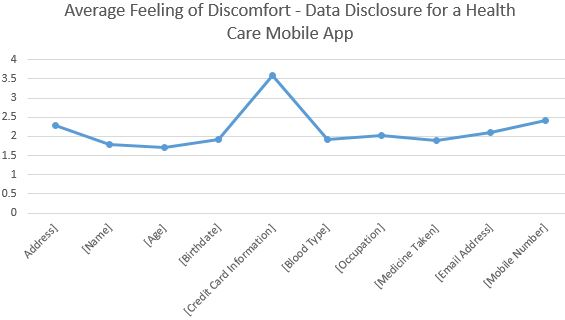
\includegraphics[width=0.5\textwidth]{Average_Health}
\caption{Feeling of Discomfort in Disclosure - Health  application}
\end{center}
\end{figure}

\begin{figure}[h]
\begin{center}
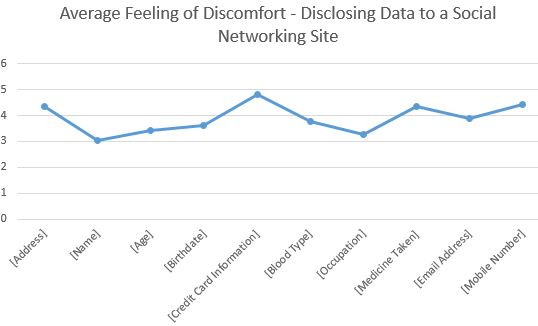
\includegraphics[width=0.5\textwidth]{Average_SocialNetworking}
\caption{Feeling of Discomfort in Disclosure - Social Networking application}
\end{center}
\end{figure}

\begin{figure}[h]
\begin{center}
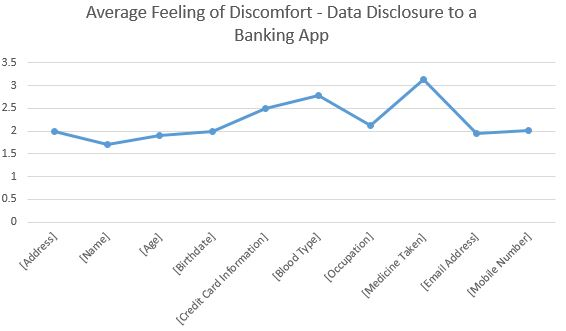
\includegraphics[width=0.5\textwidth]{Average_Banking}
\caption{Feeling of Discomfort in Disclosure - Banking application}
\end{center}
\end{figure}

The variations in the discomfort in data disclosure is discussed in detail when we discuss our results in the next section.

Then we attempted to fit our model on the raw data available (151 users and 30 instances, altogether 4530 instances). However, due to the relatively high variation of data, it was not possible to fit a model to this data set. That is the same combination of S,V, R values had multiple perceived privacy risks varying from 1 to 5. This is expected because users have very different perceived privacy risks. Therefore, we then averaged the perceived privacy risk of all 151 users to obtain 30 distinct mean perceived privacy risk values for the 30 scenarios tested. Then we used these values to observe the goodness of fit of our proposed model in Matlab. 

Table VIII shows the results when we tested different models for calculated privacy risk $P_{(i,j)}$ against the perceived privacy risk $F_d$. 

\begin{center}
\begin{table}[htbp]
\caption{Model Fitting - linear model}
\begin{center}
\begin{adjustbox}{width=0.5\textwidth} 
\begin{tabular}{|p{0.25\linewidth}|p{0.2\linewidth}|p{0.55\linewidth}|} 
\hline
Model & a (95\% CI) & Goodness of fit\\
\hline
$\frac{S_{i}^1 \times V_{(i,j)}^1}{R_{(i,j)}^1}$  & 0.24 & SSE : 67.8  $R^2$ = 0.6 RMSE = 1.5 \\
\hline
\end{tabular}
\end{adjustbox}
\end{center}
\end{table}
\end{center} 

As seen in the table VIII, that when we give the same power to all three parameters in the relationship the error is relatively high with a low R-square value. Therefore, we tried all 27 combinations of the powers 1,2 and 3 for S,V,R combinations without the combinations where all parameters got the same power. That is we ignored the combinations (1,1,1), (2,2,2) and (3,3,3). Table IX shows the results.
\begin{center}
\begin{table}[htbp]
\caption{Model Fitting}
\begin{center}
\begin{adjustbox}{width=0.5\textwidth} 
\begin{tabular}{|p{0.25\linewidth}|p{0.2\linewidth}|p{0.55\linewidth}|} 
\hline
Model & a (95\% CI) & Goodness of fit\\
\hline
 $a(  \frac{S_{i}^1 \times V_{(i,j)}^1}{R_{(i,j)}^2})$ & 0.24 &  SSE: 15.22   $R^2$ : 0.4353  RMSE : 0.7373\\
\hline
 $a(  \frac{S_{i}^1 \times V_{(i,j)}^1}{R_{(i,j)}^3}) $ & 0.21 & SSE: 16.7  $R^2$ : 0.3803  RMSE : 0.7723 \\
\hline
 $a(  \frac{S_{i}^1 \times V_{(i,j)}^2}{R_{(i,j)}^1})$ & 0.10 & SSE: 9.335 $R^2$: 0.6536  RMSE : 0.5774 \\
\hline
$a(  \frac{S_{i}^1 \times V_{(i,j)}^2}{R_{(i,j)}^2})$ & 0.08 & SSE: 12.57  $R^2$ : 0.5336  RMSE : 0.67 \\
\hline
$a(  \frac{S_{i}^1 \times V_{(i,j)}^2}{R_{(i,j)}^3})$ & 0.08 &   SSE: 14.4  $R^2$ : 0.4657  RMSE : 0.7171\\
\hline
$a(  \frac{S_{i}^1 \times V_{(i,j)}^3}{R_{(i,j)}^1})$ & 0.03 & SSE: 8.285  $R^2$ : 0.6926  RMSE : 0.544 \\
\hline
$a(  \frac{S_{i}^1 \times V_{(i,j)}^3}{R_{(i,j)}^2})$ & 0.03 & SSE: 11.73  $R^2$: 0.5646  RMSE : 0.5646 \\
\hline
 $a(  \frac{S_{i}^1 \times V_{(i,j)}^3}{R_{(i,j)}^3})$ & 0.02 &  SSE: 13.71  $R^2$: 0.4912  RMSE : 0.6998 \\
\hline
 $a(  \frac{S_{i}^2 \times V_{(i,j)}^1}{R_{(i,j)}^1})$ & 0.08 &  SSE: 13.94  $R^2$ : 0.4828  RMSE : 0.7055 \\
\hline
 $a(  \frac{S_{i}^2 \times V_{(i,j)}^1}{R_{(i,j)}^2})$ & 0.07 & SSE: 15.38  $R^2$ : 0.4294 RMSE : 0.7411  \\
\hline
$a(  \frac{S_{i}^2 \times V_{(i,j)}^1}{R_{(i,j)}^3})$ & 0.07 &  SSE: 16.45  $R^2$ : 0.3895 RMSE : 0.7666  \\
\hline
 $a(  \frac{S_{i}^2 \times V_{(i,j)}^2}{R_{(i,j)}^1})$ & 0.03 & SSE: 11.06  $R^2$ : 0.5897  RMSE : 0.6284 \\
\hline
$a(  \frac{S_{i}^2 \times V_{(i,j)}^2}{R_{(i,j)}^3})$ & 0.02 & SSE: 14.78  $R^2$ : 0.4515  RMSE : 0.7266 \\
\hline
 $a(  \frac{S_{i}^2 \times V_{(i,j)}^3}{R_{(i,j)}^1})$ &  0.01 &  SSE: 10.07  $R^2$ : 0.6264  RMSE : 0.5996 \\
\hline
 $a(  \frac{S_{i}^2 \times V_{(i,j)}^3}{R_{(i,j)}^2})$ & 0.009 & SSE: 12.74  $R^2$ : 0.5271  RMSE : 0.6746 \\
\hline
 $a(  \frac{S_{i}^2 \times V_{(i,j)}^3}{R_{(i,j)}^3})$ & 0.009 & SSE: 14.38  $R^2$ : 0.4665  RMSE : 0.7166\\
\hline
 $a(  \frac{S_{i}^3 \times V_{(i,j)}^1}{R_{(i,j)}^1})$ & 0.02 & SSE: 14.37  $R^2$ : 0.4669  RMSE : 0.7163 \\
\hline
 $a(  \frac{S_{i}^3 \times V_{(i,j)}^1}{R_{(i,j)}^2})$ & 0.02 & SSE: 15.31  $R^2$ : 0.432  RMSE : 0.7394 \\
\hline
 $a(  \frac{S_{i}^3 \times V_{(i,j)}^1}{R_{(i,j)}^3})$ & 0.02 & SSE: 16.22  $R^2$ : 0.3982  RMSE : 0.7611 \\
\hline
$a(  \frac{S_{i}^3 \times V_{(i,j)}^2}{R_{(i,j)}^1})$ & 0.009 & SSE : 11.68  $R^2$ : 0.5664  RMSE : 0.646 \\
\hline
$a(  \frac{S_{i}^3 \times V_{(i,j)}^2}{R_{(i,j)}^2})$ & 0.009 & SSE : 13.56  $R^2$ : 0.497  RMSE : 0.6958\\
\hline
 $a(  \frac{S_{i}^3 \times V_{(i,j)}^2}{R_{(i,j)}^3})$ & 0.008 & SSE: 14.86 $R^2$ : 0.4485  RMSE : 0.7286 \\
\hline
 $a(  \frac{S_{i}^3 \times V_{(i,j)}^3}{R_{(i,j)}^1})$ & 0.003 & SSE: 10.78  $R^2$ : 0.5998  RMSE : 0.6206 \\
\hline
$a(  \frac{S_{i}^3 \times V_{(i,j)}^3}{R_{(i,j)}^2})$ & 0.003 & SSE: 13.12  $R^2$ : 0.513  RMSE : 0.6846 \\
\hline
\end{tabular}
\end{adjustbox}
\end{center}
\end{table}
\end{center} 

From the above result we can see that the goodness of fit increases with the increase in of the power of visibility and decreases when the power of sensitivity and relatedness increases. Therefore, we then gradually increased the power of visibility and tested the goodness of fit while keeping the power of sensitivity and relatedness at 1.Table X shows the values we received.
\begin{center}
\begin{table}[htbp]
\caption{Model Fitting - increasing the power of visibility}
\begin{center}
\begin{adjustbox}{width=0.5\textwidth} 
\begin{tabular}{|p{0.25\linewidth}|p{0.2\linewidth}|p{0.55\linewidth}|} 
\hline
Model & a (95\% CI) & Goodness of fit\\
\hline
 $a(  \frac{S_{i}^1 \times V_{(i,j)}^4}{R_{(i,j)}^1})$ & 0.01 &  SSE: 7.872   $R^2$ : 0.7079  RMSE 0.5302\\
\hline
 $a(  \frac{S_{i}^1 \times V_{(i,j)}^5}{R_{(i,j)}^1}) $ & 0.003 & SSE: 7.723 $R^2$ : 0.7134  RMSE : 0.5252 \\
\hline
$a(  \frac{S_{i}^1 \times V_{(i,j)}^6}{R_{(i,j)}^1})$ & 0.001 & SSE : 7.682  $R^2$ : 0.7149  RMSE : 0.5238 \\
\hline
$a(  \frac{S_{i}^1 \times V_{(i,j)}^7}{R_{(i,j)}^1})$ & 0.01 &   SSE : 7.682  $R^2$ : 0.715  RMSE : 0.5238 \\
\hline
$a(  \frac{S_{i}^1 \times V_{(i,j)}^8}{R_{(i,j)}^1})$ & 0.01 & SSE : 7.693  $R^2$ : 0.7145  RMSE : 0.5242 \\
\hline
$a(  \frac{S_{i}^1 \times V_{(i,j)}^9}{R_{(i,j)}^1})$ & 4.378e-05  & SSE : 7.706  $R^2$  : 0.7141  RMSE : 0.5246 \\
\hline
\end{tabular}
\end{adjustbox}
\end{center}
\end{table}
\end{center}

We can see that the error increases again the power of visibility increases beyond 6. Therefore, the optimal relationship with the best goodness of fit is,

\[
\frac{S_{i}^1 \times V_{(i,j)}^6}{R_{(i,j)}^1}
\]

From this result it can be seen that the visibility has the largest effect on the perceived privacy risk of users. Therefore, when designing software systems, if the system could control the visibility of data in the system and communicate how visible the data would be once the user disclose data into the system, it would help reducing the perceived privacy risk of users. 

In order to further observe why users felt differently when they disclosed data in the three scenarios we described, in the next section we present the qualitative analysis of the reasons users gave.

\subsubsection{Qualitative analysis on factors that affect the feeling of discomfort in data disclosure}

Table XI gives the summary of the codes we generated through the qualitative analysis. We developed a total of 11 codes.

\begin{center}
\begin{table*}[htbp]
\caption{Issues participants faced when embedding privacy into the designs}
\begin{center}
\begin{adjustbox}{width=1\textwidth}
\begin{tabular}{|p{0.20\linewidth}|p{0.64\linewidth}|p{0.16\linewidth}|}
\hline
Code &  Representative Quotes & Coverage (out of 151)\\
\hline
Benefit to me &how it benefits myself/ how useful it is for me. & 2.64\% (4)\\
\hline
How much I need the app &  based on my requirements from the application & 7.2\%(11)\\
\hline
News I see  & by considering cyber crimes and all that & 0.66\%(1) \\
\hline
Personal experience &  I was in couple of these situations which gave me an idea & 2\%(3) \\
\hline
Personal Safety & Some data are highly confidential and could end up in a reputation and/or financial loss/  don't like to see unwanted advertisements and messages & 12\% (19)\\ 
\hline
Relevance of data to the purpose &if I don't think such applications needs the data. For instance my blood group for a banking app
 & 26\% (40)\\ 
\hline
Visibility of Data - who can see it & audience with access to the data/ as in whether I could control what others see & 12\% (19)\\ 
\hline
Sensitivity of Data & As long as the requested information is not sensitive/  some sensitive information can't be disclosed irrespective of the application
 & 15\% (23)\\ 
\hline
Transparency - knowing how the data is used & Depends on what they are going to do with the information/ when privacy is not guaranteed & 6.6\% (10)\\ 
\hline
Trust with the application & every online application cannot be trusted/ random Facebook applications are not safe & 11\% (17)\\ 
\hline
Trust with the organization & If it is a reputed or a government institution there is less doubt and more trust on data security
 & 19\% (29)\\ 
\hline
\end{tabular}
\end{adjustbox}
\end{center}
\end{table*}
\end{center}

When it comes to the properties of data, participants mentioned only sensitivity, relevance and visibility of the data items that affect their disclosure decisions. We could not identify any other attribute related to the data itself that affected the perceived privacy risk of users when they disclosed data. Participants were most concerned about the relevance of data (26\%) followed by sensitivity of data (15\%) and visibility (12\%). Nevertheless, our model showed that the visibility of data had the highest impact on the perceived privacy risk of users.

Consequently, we identified that users are concerned about the trust towards the organization that develop and publish applications (19\%). Participants said that they are comfortable sharing data as long as the application is developed and owned by a trusted organization. This was observed in the mean perceived privacy risk of users we calculated for the three application contexts. We observed a relatively low mean perceived privacy risk for the scenario with the banking app, probably because users trusted their bank more. Some participants spoke about the trust with the application itself rather than the organization (11\%). Some participants also raised concerns about personal safety (12\%). Their concerns on personal safety was two fold. One was on financial and reputation loss on data being accessed by unknown parties. The other was their concern on being subjected to unwanted marketing via phone and email. They said that they consider this as a personal threat and hence they think twice before disclosing data to any application. A small number of participants were concerned about the previous personal experience and also about the benefit of sharing the data. 

\section {Limitations}

The model we derived here does not account for the human attributes of users that affect their perceived privacy risk when interacting with software systems. Previous research has shown that the personality of users could affect the expected privacy of users in a given scenario, which impact the perceived privacy risk of users when they interact with software systems. For example, Westin's privacy personality scale identify three categories of users with different levels of privacy expectations \cite {westin1991equifax}. They have shown that users could be divided into privacy fundamentalists, who are extremely concerned about their privacy, privacy pragmatists, who understand that privacy needs to be compromised according to situations and privacy unconcerned, who are either little not concerned about their privacy. These personalities of users could affect the perceived privacy risk of users. For example, in our survey P41 said \textit{Basically I feel comfortable giving information on a need to know basis only} and P114 said \textit {nothing} implying he did not feel different disclosing data into different application settings. Consequently, there could exist other attributes such as previous experience of users, their age and the nature of work they do that may affect their perceived privacy risk. For example, P5 said \textit{With the experiences when surfing in the internet made me to answer above questions so} and P89 said \textit {I was in couple of these situations which gave me an idea to answer these questions easily}. However, in this research our focus was to model the perceived privacy risk eliminating the personality traits of a person. Therefore, by design we did not capture the privacy profile of our participants. The model we tested had an SSE value of 7.682 and an $R_{2}$ value of ~71\%. This could be taken as an acceptable goodness of fit in a human study. While the variations in the model could probably be explained by human factors, for the purpose of deriving a model for software developers to approximate the perceived privacy risk of the data used in software systems, we believe our model is appropriate.

As future work, we aim to run our study with privacy profiling of participants in order to observe how our model could cater for the privacy requirements of users with different privacy personalities. 



\section{Conclusion and Future Work}
In this research we derived and proposed a model to calculate the perceived privacy risk of users when they disclose data into software systems. We used the sensitivity of data, the visibility data gets in a system design and the relatedness of data to the system as the independent variables in the model. We then tested our model against actual perceived privacy risk of users in three different application settings. Our model shows that the visibility of a data item has the highest impact on the perceived privacy risk of users when disclosing data into software systems. Sensitivity and relatedness of data had a similar impact where sensitivity is related to privacy risk in a monotonically incrementing relationship and relatedness is in a monotonically decreasing relationship with privacy risk. The proposed model could be used when designing software systems to approximate the perceived privacy risk users would encounter when they interact with the system. Therefore, system designers could incorporate privacy messages and privacy by design in order to reduce the privacy risk of users for data items that has a higher perceived privacy risk. 



\iffalse

\begin{figure} 
\centering
\includegraphics [height=2 in,width=3 in]{Figure2.pdf}
\caption{Answer structure in a given security question \protect}
\vskip -6pt
\end{figure}
\fi

\iffalse 
Lying to a human being is a very bad thing to do, but, what if one lying to a computer to protect her privacy and keep her safe. 
\fi


\iffalse 
% no \IEEEPARstart
This demo file is intended to serve as a ``starter file''
for IEEE conference papers produced under \LaTeX\ using
IEEEtran.cls version 1.7 and later.
% You must have at least 2 lines in the paragraph with the drop letter
% (should never be an issue)
I wish you the best of success. 
\hfill mds
\hfill January 11, 2007

\subsection{Subsection Heading Here}
Subsection text here.


\subsubsection{Subsubsection Heading Here}
Subsubsection text here.
\fi




\iffalse 
\footnotesize
\bibliographystyle{abbrv}
\section{Conclusion}
The conclusion goes here. 




% conference papers do not normally have an appendix


% use section* for acknowledgement
\section*{Acknowledgment}


zzxzxz


\fi




\bibliographystyle{IEEEtran}
% argument is your BibTeX string definitions and bibliography database(s)
\bibliography{references}

\iffalse 
\begin{thebibliography}{1}

\bibitem{IEEEhowto:kopka}
H.~Kopka and P.~W. Daly, \emph{A Guide to \LaTeX}, 3rd~ed.\hskip 1em plus
0.5em minus 0.4em\relax Harlow, England: Addison-Wesley, 1999.

\end{thebibliography}




\section{Interview script}
Interview study 

\subsection*{ Demographics}

\begin{enumerate}
\item How old are you? ~\footnote{Most questions are open-ended questions}\\
\item How many people other than you live in your house?\\ 
\item What is each person's relationship to you?\\
\item What grade are you in school?\\
\end{enumerate}
\fi
\appendices

\section {Appendix A Survey Questionnaire}



% that's all folks
\end{document}



